\chapter{Einleitung}

\section{Aufgabe und Motivation}
Ziel dieses Versuches ist die experimentelle Bestimmung der Erdbeschleunigung $g$ mithilfe eines Federpendels. Hierfür wird eine Feder mit bekannter Federkonstanten $D$ durch (unterschiedliche) Massen $m$ belastet. Aus der resultierenden Schwingungsdauer $T$ lassen sich Rückschlüsse auf die Erdbeschleunigung ziehen. Der Versuch erlaubt somit, grundlegende mechanische Zusammenhänge zwischen Masse, Federkraft und Schwingungsdauer zu untersuchen.

\section{Physikalische Grundlage}
Ein Federpendel unterliegt der Hooke'schen Kraft, die proportional zur Auslenkung $x$ ist \cite{skript25,demtroeder17}:
\begin{equation}
    F = -D \, x,
\end{equation}
wobei $D$ die Federkonstante der Feder beschreibt. Die Bewegungsgleichung für das Federpendel lautet demnach:
\begin{equation}
    m \, \ddot{x} + D \, x = 0.
\end{equation}

Die Lösung dieser Differentialgleichung für die Anfangsauslenkung $x_0$ zum Zeitpunkt $t = 0$ ergibt:
\begin{equation}
    x(t) = x_0 \, \cos(\omega t),
\end{equation}
wobei die Kreisfrequenz $\omega$ gegeben ist durch
\begin{equation}
    \omega = \sqrt{\frac{D}{m}}.
\end{equation}

Da die Periodendauer $T$ im Zusammenhang mit der Kreisfrequenz $\omega$ steht, lässt sich folgendes berechnen:
\begin{equation}
    T = \frac{2 \pi}{\omega} = 2 \pi \sqrt{\frac{m}{D}}.
\end{equation}

Für die statische Auslenkung $x_\text{stat}$, also dem Equilibrium, der Feder unter der Gewichtskraft $mg$ gilt:
\begin{equation}
    x_\text{stat} = \frac{mg}{D}.
\end{equation}

Durch Messung der Schwingungsdauer $T$ für unterschiedliche Massen $m$ kann zunächst die Federkonstante $D$ überprüft und anschließend die Erdbeschleunigung $g$ bestimmt werden. 
\subsubsection*{Skizze des Veruaufbaus}
\begin{figure}[h!]
    \centering
    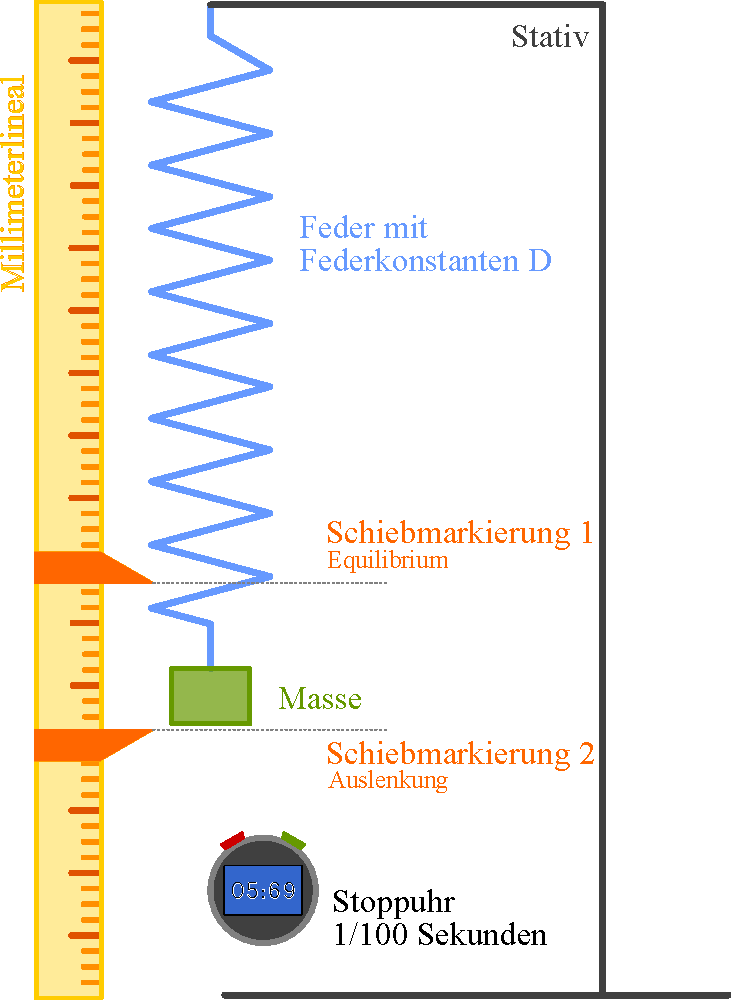
\includegraphics[width=\columnwidth]{img/11/Versuchsaufbau.pdf}
    \caption{Skizze des Versuchsaufbaus \newline und der Ausrüstung}
    \label{fig:versuchsaufbau}
\end{figure}
